\section{Benchmarks}

  We benchmark state of the art 2D networks for both object--detection
  and semantical segmentation as well as 3D networks.

  First, we demonstrate the near--linear scalability of our approach,
  regardless of the layer shape.  We show that our approach has the
  same utilization for all of them.

  Secondly, we compare the speed of our approach to alternative 2D
  primitives -- specifically CcT, MKL--DNN and MKL--2017.  We show
  that our approach is competitive, over--performing the next bet
  competitor by a small margin on Xeon and under--performing by a
  small margin on the KNL for 2D object--detection.  However, for
  semantical segmentation, we greatly outperform all competitors on
  both Xeon and Xeon Phi.

  Finally, we compare the speed of 3D networks to state of the art 3D
  primitives for the GPU.

  \subsection{Experimental setup}

  Describe the machines

  \begin{table}
    \begin{center}
      \begin{tabular}{lr}
        \hline
        Processor & GFLOPs/s\\
        \hline
        i7-6700K (Skylake) & 512\\
        4-way E7-8890v3 (Haswell) & 5760\\
        Xeon Phi 7210 & 4505.6\\
        Titan X (Maxwell) & 6600\\
        Titan X (Pascal) & 11000\\
        \hline
      \end{tabular}
    \end{center}
    \caption{Machines used for the benchmarks}
  \end{table}

  \subsection{Benchmarked networks}

  Describe the networks

  \begin{enumerate}
  \item VGG--A
  \item U--Net
  \item 3D network from \url{https://arxiv.org/pdf/1412.0767.pdf}
  \end{enumerate}


%%   \begin{table*}
%%   \begin{center}
%%     \begin{tabular}{llrrrrrrrr}
%%       \hline
%%       Layer & Topology & MKL-DNN (fwd) & MKL-DNN (bwd) & ZNNphi (fwd) & ZNNPhi (bwd) & CcT (fwd) & CcT (bwd) & MKL2017 (fwd) & MKL 2017 (bwd)\\
%%       \hline
%%       Conv1 & 3x224x224   -> 64x224x224 &  49.3624 & 64.3649 &  & FWD + 11.5648 & 82.1643 & 146.155 & 17.8144 & 3356.7\\
%%       Conv2 & 64x112x112  -> 128x112x112 & 79.1275 & 196.401 & 42.875 & 79.0901 & 141.209 & 317.833 & 43.7455 & 99.285\\
%%       Conv3 & 128x56x56   -> 256x56x56 & 42.3746 & 106.796 & 29.3154 & 61.5185 & 118.521 & 194.27 & 29.9454 & 78.4889\\
%%       Conv4 & 256x56x56   -> 256x56x56 & 101.276 & 322.293 & 54.0394 & 115.0899 & 263.519 & 395.418 & 58.5886 & 158.027\\
%%       Conv5 & 256x28x28   -> 512x28x28 & 44.226 & 203.507 & 27.9326 & 60.6804 & 92.5641 & 233.93 & 27.3278 & 76.2447\\
%%       Conv6 & 512x28x28   -> 512x28x28 & 89.8072 & 466.538 & 51.2921 & 115.6594 & 196.814 & 466.345 & 51.8565 & 149.924\\
%%       Conv7 & 512x14x14   -> 512x14x14 & 21.0151 & 175.31 & 15.3210 & 33.2321 & 47.4143 & 237.32 & 14.7956 & 37.1315\\
%%       Conv8 & ------ SAME ------ & 23.0235 & 173.278 & 15.2122 & 32.9128 & 43.3761 & 251.593 & 15.0066 & 37.0637\\
%%       \hline
%%     \end{tabular}
%%   \end{center}
%%   \end{table*}


%%   \begin{table*} \centering
%%     \begin{tabular}{cl||cccccc||cc|cc|cc|cc||cc|cc|cc||cc||}
%%       & & \multicolumn{6}{c}{Layer Description} & \multicolumn{8}{c}{Haswell}
%%       & \multicolumn{6}{c}{Knights Landing} & \multicolumn{2}{c}{Titan X GPU} \\
%%         & & \rot{Batch Size} & \rot{Input Channels} & \rot{Output Channels} & \rot{Image H/W}
%%         & \rot{Padding H/W} & \rot{Kernel H/W}
%%         & \rot{Forward} & \rot{Bwd+Update}
%%         & \rot{Forward} & \rot{Bwd+Update}
%%         & \rot{Forward} & \rot{Bwd+Update}
%%         & \rot{Forward} & \rot{Bwd+Update}
%%         & \rot{Forward} & \rot{Bwd+Update}
%%         & \rot{Forward} & \rot{Bwd+Update}
%%         & \rot{Forward} & \rot{Bwd+Update}
%%         & \rot{Forward} & \rot{Bwd+Update} \\
%%         \hline
%%         \multirow{6}{*}{{VGG-A}}x
%%         & Conv2             & 64 & 64   & 128  & 112   & 1 & 3  &  \\
%%         & Conv3             & 64 & 128  & 256  &  56   & 1 & 3  &  \\
%%         & Conv4             & 64 & 256  & 256  &  56   & 1 & 3  &  \\
%%         & Conv5             & 64 & 256  & 512  &  28   & 1 & 3  &  \\
%%         & Conv6             & 64 & 512  & 512  &  28   & 1 & 3  &  \\
%%         & Conv7             & 64 & 512  & 512  &  14   & 1 & 3  &  \\
%%         \hline
%%         \multirow{9}{*}{{U--Net}}
%%         & Conv1b             & 1 & 64   & 64   & 570  & 0 & 3 &\\
%%         & Conv2a             & 1 & 64   & 128  & 284  & 0 & 3 &\\
%%         & Conv2b             & 1 & 128  & 128  & 282  & 0 & 3 &\\
%%         & Conv3a             & 1 & 128  & 256  & 140  & 0 & 3 &\\
%%         & Conv3b             & 1 & 256  & 256  & 138  & 0 & 3 &\\
%%         & Conv4a             & 1 & 256  & 512  & 68   & 0 & 3 &\\
%%         & Conv4b             & 1 & 512  & 512  & 66   & 0 & 3 &\\
%%         & Conv5a             & 1 & 512  & 1024 & 32   & 0 & 3 &\\
%%         & Conv5b             & 1 & 120  & 1024 & 30   & 0 & 3 &\\
%%         \bottomrule
%%     \end{tabular}
%%     \caption{Some caption}
%% \end{table*}


%%   \begin{figure*} \centering
%%     \small
%%     \begin{tabular}{cr !{\vrule width0.8pt} cc|cc|cc|cc !{\vrule width0.8pt} cc|cc|cc !{\vrule width0.8pt} cc }
%%       & & \multicolumn{8}{c !{\vrule width0.8pt} }{\textbf{Haswell}} & \multicolumn{6}{c !{\vrule width0.8pt}}{\textbf{Knights Landing}}
%%       & \multicolumn{2}{c}{\textbf{Titan X GPU}} \\
%%       \hline
%%       & & \multicolumn{2}{c|}{MKL-DNN} & \multicolumn{2}{c|}{MKL-2017}
%%       & \multicolumn{2}{c|}{CcT} & \multicolumn{2}{c !{\vrule width0.8pt}}{ZNNPhi}
%%       & \multicolumn{2}{c|}{MKL-DNN} & \multicolumn{2}{c|}{MKL-2017}
%%       & \multicolumn{2}{c !{\vrule width0.8pt}}{ZNNPhi} & \multicolumn{2}{c}{CuDNNv4} \\
%%       %\hline

%%       &  & Fwd & Bwd & Fwd & Bwd& Fwd & Bwd& Fwd & Bwd& Fwd & Bwd& Fwd & Bwd& Fwd & Bwd& Fwd & Bwd\\
%%       \hline
%%       \multirow{6}{*}{\rotatebox{90}{\textbf{VGG-A}}}
%%       & C2 & 79.12 & 196.4 & 42.87 & 79.09 & 141.2 & 317.8 & 43.74 & 99.28 & 79.12 & 196.4 & 42.87 & 79.09 & 141.2 & 317.8 & 43.74 & 99.28 \\
%%       & C3 & 79.12 & 196.4 & 42.87 & 79.09 & 141.2 & 317.8 & 43.74 & 99.28 & 79.12 & 196.4 & 42.87 & 79.09 & 141.2 & 317.8 & 43.74 & 99.28 \\
%%       & C4 & 79.12 & 196.4 & 42.87 & 79.09 & 141.2 & 317.8 & 43.74 & 99.28 & 79.12 & 196.4 & 42.87 & 79.09 & 141.2 & 317.8 & 43.74 & 99.28 \\
%%       & C5 & 79.12 & 196.4 & 42.87 & 79.09 & 141.2 & 317.8 & 43.74 & 99.28 & 79.12 & 196.4 & 42.87 & 79.09 & 141.2 & 317.8 & 43.74 & 99.28 \\
%%       & C6 & 79.12 & 196.4 & 42.87 & 79.09 & 141.2 & 317.8 & 43.74 & 99.28 & 79.12 & 196.4 & 42.87 & 79.09 & 141.2 & 317.8 & 43.74 & 99.28 \\
%%       & C7 & 79.12 & 196.4 & 42.87 & 79.09 & 141.2 & 317.8 & 43.74 & 99.28 & 79.12 & 196.4 & 42.87 & 79.09 & 141.2 & 317.8 & 43.74 & 99.28 \\
%%       \hline
%%       \multirow{9}{*}{\rotatebox{90}{\textbf{U-Net}}}
%%       & C1b & 79.12 & 196.4 & 42.87 & 79.09 & 141.2 & 317.8 & 43.74 & 99.28 & 79.12 & 196.4 & 42.87 & 79.09 & 141.2 & 317.8 & 43.74 & 99.28 \\
%%       & C2a & 79.12 & 196.4 & 42.87 & 79.09 & 141.2 & 317.8 & 43.74 & 99.28 & 79.12 & 196.4 & 42.87 & 79.09 & 141.2 & 317.8 & 43.74 & 99.28 \\
%%       & C2b & 79.12 & 196.4 & 42.87 & 79.09 & 141.2 & 317.8 & 43.74 & 99.28 & 79.12 & 196.4 & 42.87 & 79.09 & 141.2 & 317.8 & 43.74 & 99.28 \\
%%       & C3a & 79.12 & 196.4 & 42.87 & 79.09 & 141.2 & 317.8 & 43.74 & 99.28 & 79.12 & 196.4 & 42.87 & 79.09 & 141.2 & 317.8 & 43.74 & 99.28 \\
%%       & C3b & 79.12 & 196.4 & 42.87 & 79.09 & 141.2 & 317.8 & 43.74 & 99.28 & 79.12 & 196.4 & 42.87 & 79.09 & 141.2 & 317.8 & 43.74 & 99.28 \\
%%       & C4a & 79.12 & 196.4 & 42.87 & 79.09 & 141.2 & 317.8 & 43.74 & 99.28 & 79.12 & 196.4 & 42.87 & 79.09 & 141.2 & 317.8 & 43.74 & 99.28 \\
%%       & C4b & 79.12 & 196.4 & 42.87 & 79.09 & 141.2 & 317.8 & 43.74 & 99.28 & 79.12 & 196.4 & 42.87 & 79.09 & 141.2 & 317.8 & 43.74 & 99.28 \\
%%       & C5a & 79.12 & 196.4 & 42.87 & 79.09 & 141.2 & 317.8 & 43.74 & 99.28 & 79.12 & 196.4 & 42.87 & 79.09 & 141.2 & 317.8 & 43.74 & 99.28 \\
%%       & C5b & 79.12 & 196.4 & 42.87 & 79.09 & 141.2 & 317.8 & 43.74 & 99.28 & 79.12 & 196.4 & 42.87 & 79.09 & 141.2 & 317.8 & 43.74 & 99.28 \\
%%       \hline
%%       \multirow{8}{*}{\rotatebox{90}{\textbf{VD2D3D}}}
%%       & C1b & 79.12 & 196.4 & 42.87 & 79.09 & 141.2 & 317.8 & 43.74 & 99.28 & 79.12 & 196.4 & 42.87 & 79.09 & 141.2 & 317.8 & 43.74 & 99.28 \\
%%       & C1c & 79.12 & 196.4 & 42.87 & 79.09 & 141.2 & 317.8 & 43.74 & 99.28 & 79.12 & 196.4 & 42.87 & 79.09 & 141.2 & 317.8 & 43.74 & 99.28 \\
%%       & C2a & 79.12 & 196.4 & 42.87 & 79.09 & 141.2 & 317.8 & 43.74 & 99.28 & 79.12 & 196.4 & 42.87 & 79.09 & 141.2 & 317.8 & 43.74 & 99.28 \\
%%       & C2b & 79.12 & 196.4 & 42.87 & 79.09 & 141.2 & 317.8 & 43.74 & 99.28 & 79.12 & 196.4 & 42.87 & 79.09 & 141.2 & 317.8 & 43.74 & 99.28 \\
%%       & C3a & 79.12 & 196.4 & 42.87 & 79.09 & 141.2 & 317.8 & 43.74 & 99.28 & 79.12 & 196.4 & 42.87 & 79.09 & 141.2 & 317.8 & 43.74 & 99.28 \\
%%       & C3b & 79.12 & 196.4 & 42.87 & 79.09 & 141.2 & 317.8 & 43.74 & 99.28 & 79.12 & 196.4 & 42.87 & 79.09 & 141.2 & 317.8 & 43.74 & 99.28 \\
%%       & C4a & 79.12 & 196.4 & 42.87 & 79.09 & 141.2 & 317.8 & 43.74 & 99.28 & 79.12 & 196.4 & 42.87 & 79.09 & 141.2 & 317.8 & 43.74 & 99.28 \\
%%       & C4b & 79.12 & 196.4 & 42.87 & 79.09 & 141.2 & 317.8 & 43.74 & 99.28 & 79.12 & 196.4 & 42.87 & 79.09 & 141.2 & 317.8 & 43.74 & 99.28 \\
%%       \hline

%%     \end{tabular}
%%     \caption{Some caption}
%% \end{figure*}


  \begin{figure*} \centering
    \small
    \setlength\tabcolsep{0.5pt}
    \begin{tabular}{ >{\centering\arraybackslash}c ccccccl }
      & \multicolumn{2}{c}{\textbf{Skylake}}
      & \multicolumn{2}{c}{\textbf{Haswell}}
      & \multicolumn{2}{c}{\textbf{Knights Landing}} & \\
      \hline
      & Forward & Update & Forward & Update & Forward & Update & \\
      \hline
      \rotatebox{90}{\qquad \textbf{VGG-A}}
      & 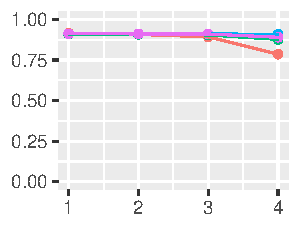
\includegraphics[height=2.4cm]{fig/vgg-fwd-skylake}
      & 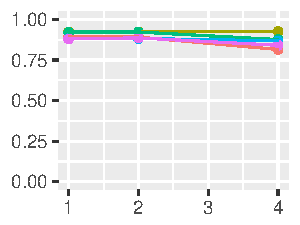
\includegraphics[trim=8mm 0mm 0mm 0mm,clip,height=2.4cm]{fig/vgg-upd-skylake}
      & 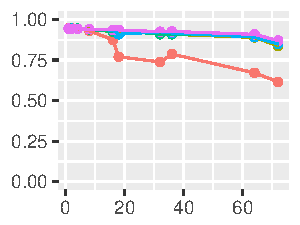
\includegraphics[trim=8mm 0mm 0mm 0mm,clip,height=2.4cm]{fig/vgg-fwd-haswell}
      & 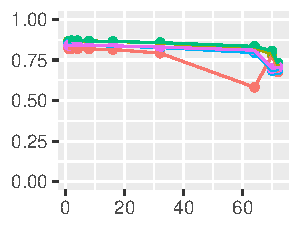
\includegraphics[trim=8mm 0mm 0mm 0mm,clip,height=2.4cm]{fig/vgg-upd-haswell}
      & 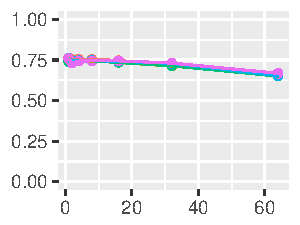
\includegraphics[trim=8mm 0mm 0mm 0mm,clip,height=2.4cm]{fig/vgg-fwd-knl}
      & 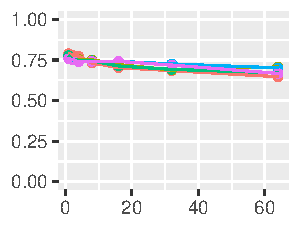
\includegraphics[trim=8mm 0mm 0mm 0mm,clip,height=2.4cm]{fig/vgg-upd-knl}
      & 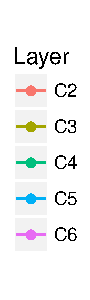
\includegraphics[height=2.4cm]{fig/vgg-legend} \\
      \hline
      \rotatebox{90}{\qquad \textbf{U-Net}}
      & 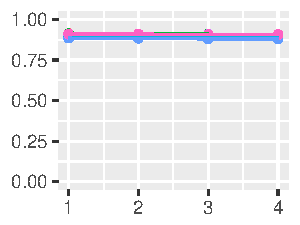
\includegraphics[height=2.4cm]{fig/unet-fwd-skylake}
      & 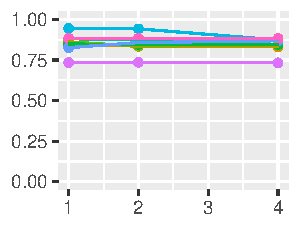
\includegraphics[trim=8mm 0mm 0mm 0mm,clip,height=2.4cm]{fig/unet-upd-skylake}
      & 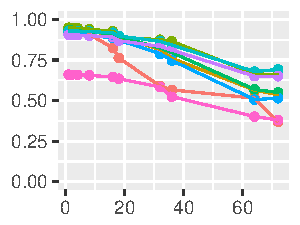
\includegraphics[trim=8mm 0mm 0mm 0mm,clip,height=2.4cm]{fig/unet-fwd-haswell}
      & 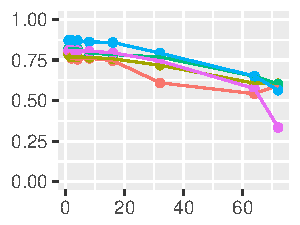
\includegraphics[trim=8mm 0mm 0mm 0mm,clip,height=2.4cm]{fig/unet-upd-haswell}
      & 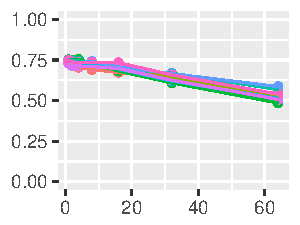
\includegraphics[trim=8mm 0mm 0mm 0mm,clip,height=2.4cm]{fig/unet-fwd-knl}
      & 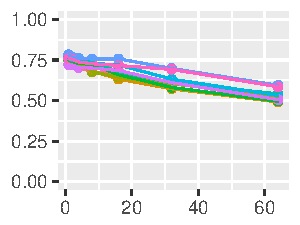
\includegraphics[trim=8mm 0mm 0mm 0mm,clip,height=2.4cm]{fig/unet-upd-knl}
      & 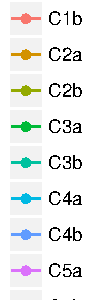
\includegraphics[height=2.4cm]{fig/unet-legend} \\
      \hline
      \rotatebox{90}{\qquad \textbf{C3D}}
      & 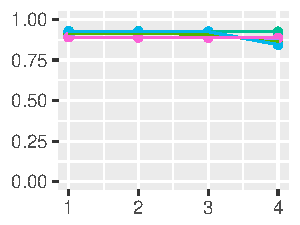
\includegraphics[height=2.4cm]{fig/d3d-fwd-skylake}
      & 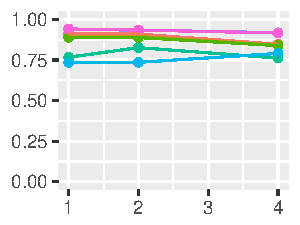
\includegraphics[trim=8mm 0mm 0mm 0mm,clip,height=2.4cm]{fig/d3d-upd-skylake}
      & 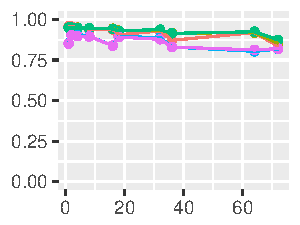
\includegraphics[trim=8mm 0mm 0mm 0mm,clip,height=2.4cm]{fig/d3d-fwd-haswell}
      & 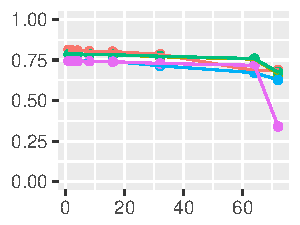
\includegraphics[trim=8mm 0mm 0mm 0mm,clip,height=2.4cm]{fig/d3d-upd-haswell}
      & 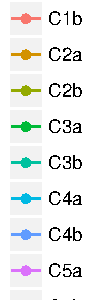
\includegraphics[trim=8mm 0mm 0mm 0mm,clip,height=2.4cm]{fig/demo}
      & 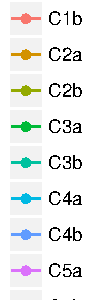
\includegraphics[trim=8mm 0mm 0mm 0mm,clip,height=2.4cm]{fig/demo}
      & 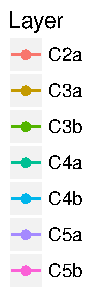
\includegraphics[height=2.4cm]{fig/d3d-legend} \\
      \hline

    \end{tabular}
    \caption{Some caption}
\end{figure*}
